\section{Normal Estimation}

Two functions are provided to estimate the normal direction of the inferred surface at each point af an input point set. In both cases the result is an unoriented normal vector for each input point.

Function \ccc{CGAL::jet_estimate_normals()} estimates the normal direction at each point from the input set by fitting a jet surface over its $k$ nearest neighbors. The default jet is a quadric surface. This algorithm is well suited to point sets scattered over curved surfaces.

Function \ccc{CGAL::pca_estimate_normals()} estimates the normal direction at each point from the set by linear least squares fitting of a plane over its $k$ nearest neighbors. This algorithm is simpler and faster than \ccc{CGAL::jet_estimate_normals()}.

\ccRefIdfierPage{CGAL::jet_estimate_normals}  \\
\ccRefIdfierPage{CGAL::pca_estimate_normals}  \\

% % Insert image pca_estimate_normals.jpg/eps
% \begin{center}
%     \label{Point_set_processing_3-fig-pca_estimate_normals}
%     % Image
%     \begin{ccTexOnly}
%         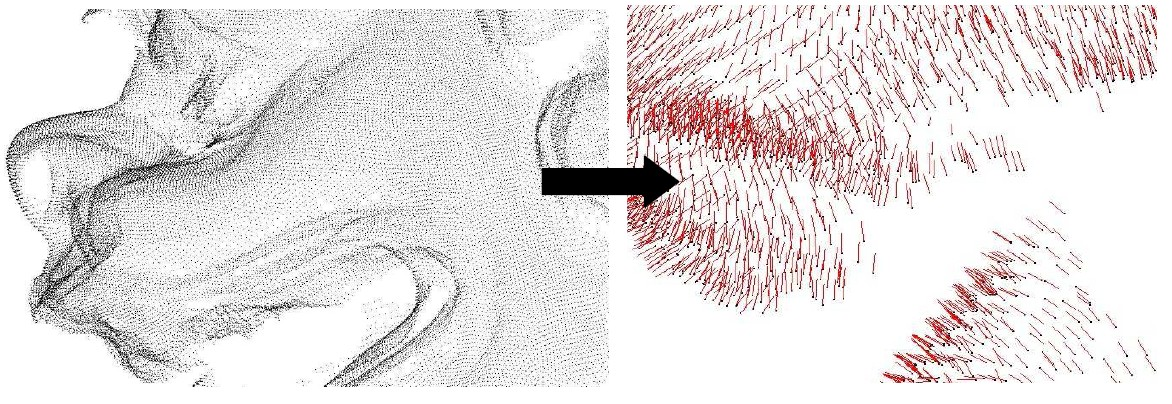
\includegraphics[width=0.9\textwidth]{Point_set_processing_3/pca_estimate_normals} % omit .eps suffix
%     \end{ccTexOnly}
%     \begin{ccHtmlOnly}
%         <img width="90%" border=0 src="./pca_estimate_normals.jpg"><P>
%     \end{ccHtmlOnly}
%     % Title
%     \begin{figure}[h]
%         \caption{Normal estimation by Principal Components Analysis}
%     \end{figure}
% \end{center}

\section{Normal Orientation}

Function \ccc{CGAL::mst_orient_normals()} orients the normals of a set of points with unoriented normals using the method described by Hoppe et al. in \emph{Surface reconstruction from unorganized points} \cite{cgal:hddms-srup-92}. More specifically, this method constructs a Riemannian graph over the input points (the graph of the $K$ nearest neighbor points) and propagates a seed normal orientation within a minimum spanning tree computed over the graph with the Boost graph library. The result is an oriented normal vector for each input point with normal.

\ccRefIdfierPage{CGAL::mst_orient_normals}  \\

% Insert image mst_orient_normals.jpg/eps
\begin{center}
    \label{Point_set_processing_3-fig-mst_orient_normals}
    % Image
    \begin{ccTexOnly}
        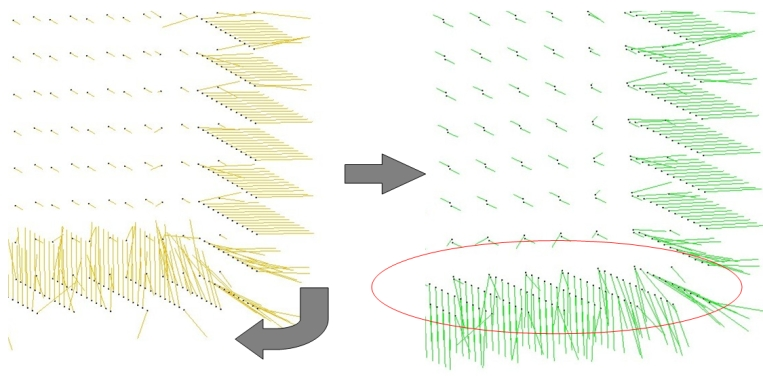
\includegraphics[width=1.0\textwidth]{Point_set_processing_3/mst_orient_normals} % omit .eps suffix
    \end{ccTexOnly}
    \begin{ccHtmlOnly}
        <img width="100%" border=0 src="./mst_orient_normals.jpg"><P>
    \end{ccHtmlOnly}
    % Title
    \begin{figure}[h]
        \caption{Normal orientation of a sampled cube surface.
                 Left: unoriented normals.
                 Right: oriented normals.}
    \end{figure}
\end{center}

The following example reads a point set from a file, estimates the normals through PCA over the 7 nearest neighbors and orient the normals:
\ccIncludeExampleCode{Point_set_processing_3/normals_example.cpp}


